\documentclass[12pt]{IEEEtran}

\usepackage[tight,footnotesize]{subfigure}

\ifCLASSINFOpdf
  \usepackage[pdftex]{graphicx}
  \graphicspath{{./images/}}
\else
\fi
\usepackage{algorithmic}
\usepackage[boxed]{algorithm}
\usepackage[cmex10]{amsmath}
\usepackage[a4paper]{ geometry}
\geometry{top=0.7in, bottom=0.7in, left=0.7in, right=0.7in}


\hyphenation{op-tical net-works semi-conduc-tor}

\begin{document}
	
\title{Individual Report 5}

\author{Calum Jackson (s0812597) - 
SDP Group 12}

\maketitle

%\numberwithin{equation}{section}
%\IEEEpeerreviewmaketitle
%\pagebreak

\section{Introduction}
This report, the last in the series, will document my contributions to the SDP project. I will begin by outlining how the team planned to tackle the project, and continue by explaining how I contributed to meeting our goals, finally concluding on my efforts and the teams efforts as a whole.\\
Our team decided to split the project into the following 4 tasks:
\begin{itemize}
\item Robot Construction
\item Building a GUI and Simulator
\item Creating a Strategy
\item Implementing a Vision System
\end{itemize}

I began by working in robot construction, and later moved into creating the playing strategy for the robot. I was also involved in large amounts of testing on the robot, and helped create and present the final day presentation.

\section{Robot Construction}
The team chose Lejos as the most suitable programming language for the NXT brick, so Marc and I began by creating a basic robot model and flashing the NXT firmware to the brick, which allowed other team members to test their initial programs on the robot. % and get to grips with the programming task ahead of them. \\
The teams aim for the robot was to have a fast, lightweight robot, giving a speed advantage over the other robots. I researched into gears, and discovered a 3 - 1 gear ratio would make our robot up to three times faster than if the wheels were connected directly to the motors\footnote{http://www.ecst.csuchico.edu/\%7Ejuliano/csci224/Slides/03\%20-\%20Gears\%20Pulleys\%20Wheels\%20Tires.pdf}. Having set-up gears up on the robot (Figure 1), I found they did affect the straight line ability of the robot, as shown below:
\begin{table}[ht]
\caption{Distance off-line (Running for 10seconds)}
\centering
\begin{tabular}{c c}
\hline\hline
Speed (rpm) & Off-Centre (mm) \\
1.5 & 82 \\
3 & 216 \\
4.5 & 850 \\
6 & N/A - Span in Circles \\
\hline\hline
\end{tabular}
\label{table:offline}
\end{table}

As shown, increased speeds led to massive offsets while travelling in a straight line. After testing multiple different options, including changing caster wheels, using ball-bearings, and putting the motors at the front, back and centre of the robot, eventually I found that the robot would diverge from its path whilst moving forwards, but would travel in a relatively straight line whilst reversing. Therefore a simple solution was to switch the direction which the motors faced (i.e. motors reversed $\rightarrow$ robot moved forward, and vice-versa). This led to much improved results:

\begin{table}[ht]
\caption{Distance off-line 2 (Running for 10seconds)}
\centering
\begin{tabular}{c c}
\hline\hline
Speed (rpm) & Off-Centre (mm) \\
1.5 & 0 \\
3 & 4 \\
4.5 &  10\\
6 & 46\\
\hline\hline
\end{tabular}
\label{table:online}
\end{table}

These reduced discrepancies could be managed by the programming of the movement. \linebreak

Further to this, I horizontally mounted the motors to lower the robots centre of gravity, repositioned the kicker motor to keep weight central whilst elevating the connection to the kicker to increase the kickers momentum whilst kicking (increased kicking distance by about 1m), built large amounts of the chassis (moving through a number of different designs), and added touch sensors to the front of the robot. \linebreak

Finally, numerous structural reinforcements were made to the robot to compensate for our robot being lighter than other robots and more susceptible to damage when being hit by other robots, and to compensate for the extra pressure put on the chassis by the increased amounts of torque and speed created by the use of gears. I feel the robot did have a distinct speed advantage, especially coupled with the potential fields movement algorithm, which utilised the robots speed efficiently, as well as being very structurally strong, contending with other robots without issues. Plus - the robot looked cool! (Figures 2-3)

\section{Strategy}

This was another section to which I was a main contributor. The main focus was to create an attacking strategy which would utilise the speed of the robot. The strategy was split into two sections, of which I worked on the high level areas (where the robot will move to, when to kick, dribble etc) as opposed to the lower level areas (coding the movement of the robot). Juozas and I began by creating a simple state system strategy, which checked the current on-pitch situation (using the data sent from the camera) and decided the appropriate strategy to run. The state system approach was used as new states could be added easily, allowing for multiple strategies, and the state system would identify the situation on the pitch each time new data was sent from the vision system. \\

Our strategy was based on defining a point to move towards. A point class had previously been created, holding the x,y co-ordinates of the point on the pitch. The class was extended to create the robot, ball, goal, and any other necessary point classes for use in the strategy. 

I calculated an optimum point (Algorithm 1), which would be a defined distance behind the ball at the same angle as the ball to goal angle, such that the robot would move to this point, and then to the ball, to ensure the robot was facing the goal when it reached the ball. This worked well in practice, working everytime when the robot was behind the ball, and 9/10 times when the robot was inbetween the goal and the ball (i.e. had to navigate around the ball).

%To calculate the angle between the ball and the goal, I created a function which used the following formula: \[angle = atan2( (y_{2} - y_{1}), (x_{2} - x_{1}) ) \] where the $ball = (x_{1}, y_{1})$ and the $goal Centre = (x_{2}, y_{2})$.

\begin{algorithm}
\caption{Caclulate Optimum Point}
\begin{algorithmic}[1]
\STATE $threshold \gets 70$
\STATE $(x_{1}, y_{1}) \gets ball (x, y)$
\STATE $(x_{2}, y_{2}) \gets goal (x, y)$
\STATE $ballGoalAngle = atan2( (y_{2} - y_{1}), (x_{2} - x_{1}) )$
%\STATE $hyp = \sqrt{\alpha^{2} + threshold^{2}}$
%\STATE $\theta = \sin(\frac{100}{hyp})$
\STATE $xOffset = threshold(\cos(ballGoallAngle)$
\STATE $yOffset = threshold(\sin(ballGoalAngle))$
\STATE $(x_{3}, y_{3}) = (x_{1} - xOffset, y_{1} - yOffset)$
\RETURN $(x_{3}, y_{3})$
\end{algorithmic}
\end{algorithm}

I later abstracted this function to a higher level, modifying the function to take any two points and return the angle between them, to increase its range and decrease repetition of similar code. \\

The next target was to be able to navigate around objects. Points were used again, as I created a function which would calculate an avoidance point at a $90^{\circ}$ angle and a defined distance from the object to avoid. The function (Algorithm 2) would return the avoidance point, which the robot would move towards. 
This function was dynamic, and the point would move as the robot moved, allowing the robot to navigate the object more smoothly.\\

\begin{center}
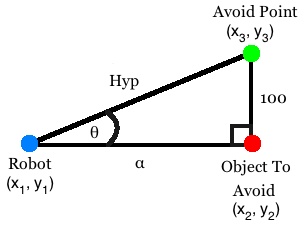
\includegraphics[scale=0.6]{AvoidPoints.png}\\
\end{center}

\begin{algorithm}
\caption{Caclulate Avoid Point}
\begin{algorithmic}[1]
\STATE $threshold \gets 100$
\STATE $(x_{1}, y_{1}) \gets Robot (x, y)$
\STATE $(x_{2}, y_{2}) \gets Object To Avoid (x, y)$
\STATE $\alpha = \sqrt{(x_{2} - x_{1})^{2} + (y_{2} - y_{1})^{2}}$
\STATE $hyp = \sqrt{\alpha^{2} + threshold^{2}}$
\STATE $\theta = \sin(\frac{100}{hyp})$
\STATE $xOffset = hyp(\cos\theta)$
\STATE $yOffset = hyp(\sin\theta)$
\STATE $(x_{3}, y_{3}) = (x_{1} + xOffset, y_{1} + yOffset)$
\RETURN $(x_{3}, y_{3})$
\end{algorithmic}
\end{algorithm}

Again, this function was abstracted to a higher level to calculate the avoidance point for any object, as the robot may need to avoid a ball or a robot. This abstraction was useful for the function I created to avoid the ball when moving the robot to get to the correct side of the ball (so the ball would be between the robot and the goal we were attacking). An example of object and ball avoidance is shown in Figure 4. \linebreak

Alongside these additions, I implemented functions which decided if the ball was in more difficult positions, such as being close to the walls or in the corners (for use in the state system), allowing different strategies to be brought in to deal with these situations, and adapted all of the strategies to readjust to a change in the goal we were attacking.
Finally, Behzad and I integrated the potential fields movement algorithm and higher level strategies, generating a fully functional strategic movement system. \linebreak

I feel a more precise shooting system (i.e. being able to shoot directly into the corners of the goal) and a defensive strategy would have improved our performance in the final competition, as a number of shots were saved in the centre of the goal, and we had no real strategy to deal with the opponent having possession, and whilst usually the attacking strategy would cover most defensive situations, we were found out once or twice in the final game. Other than these faults, the strategies worked successfully, and made good use of the robots speed.

\section{Testing}
The team's target for testing was to find bugs in the robots performance, and to check the code was performing as expected. The simulator was useful for large amounts of testing of the strategy, but I also tested each new section of code on the robot to ensure it would work correctly in real situations. I helped with the extensive testing done on the potential fields movement algorithm, as this was difficult to implement and did not perform as expected on the pitch compared to simulations (i.e. the robot would spin in circles on the pitch). 

\section{Friendly Tournaments}
During the friendly tournaments I aimed to get a good view of our robot in competition and find any bugs which had not shown up in testing. During these matches I found issues such as that the robot would have difficulty when the ball was close to the walls, or in corners. These bugs were rectified by adding new strategies (such as the GetBallFromWall strategy, which lead to a goal in our final game), and believe the friendly observations were an important part of our progress.


\section{Final Tournament}
The final matches came with disappointment, as myself and the rest of the team had high hopes for our robot, which were unfortunately brought crashing down in a 3-1 loss in the quarter-finals. We encountered unforeseen problems in that our vision could not reproduce the high frame rates we consistently had throughout the semester, and as our strategy reacted to the frames being processed, our robot ran at a much slower rate. Despite still playing fairly well, our robot failed to convert numerous chances, missing 2 penalties, and lost a match I feel could easily have been won. I still believe our robot is capable of actively competing with many of the robots who placed above us.

\section{Teamwork Contributions}
Throughout the project the goal for teamwork and communication was to keep all team members up to date with work being done on any part of the robot, and make sure members knew what their tasks were. I contributed to this by adding updates to the team website\footnote{https://sites.google.com/site/edisdp12/} every-time I worked on the robot or code, mentioning areas which weren't finished and areas which could be improved with possible additions. \linebreak

I also commented the code thoroughly to help other team-mates understand it, and constantly added TODO's to make sure tasks were not forgotten and to allow other team-mates to see how they could contribute. Additionally, during team meetings I regularly contributed ideas for future improvements across a range of areas including how to improve the robots structure and additional areas to be added to the strategy. \linebreak

I feel these contributions were all very useful in the project, and looking at all other team-mates contributions allowed me to see how the whole project was progressing and notify other team members on how to improve their sections, and vice versa.

\section{Conclusion}
Throughout this project the goal was to build a fast, lightweight robot that could compete well against other robots. Through construction I helped create a robot which was fast (at least twice as fast as most other robots) and lightweight. The robots speed was utilised effectively through the strategy and the Potential Fields movement algorithm. \linebreak

I feel one of the major breakthroughs of this project was that we managed to work well as a team, and was one of the main factors in allowing us to create a competitive robot. I also believe teamwork was one of the more challenging and enjoyable aspects of the project. On top of this, I learnt how to use SVN effectively, that robot construction is time consuming and cantankerous, and that effort (just about) reaps rewards - in this case, a lean, mean, goal scoring machine!


\newpage

\section{Appendix}

\begin{center}

\begin{figure}[htp]
\includegraphics[scale=0.2]{Pictures/gears.png}
\caption{Gears}
\end{figure}

\begin{figure}[htp]
\includegraphics[scale=0.3]{Pictures/finalRobot.jpg}
\caption{Final Robot 1}
\end{figure}

\begin{figure}[htp]
\includegraphics[scale=0.05]{Pictures/finalRobot2.jpg}
\caption{Final Robot 2}
\end{figure}

\begin{figure}[htp]
\includegraphics[scale=0.2]{Pictures/Part1-2.png}\\
\includegraphics[scale=0.2]{Pictures/Part2-2.png}\\
\includegraphics[scale=0.2]{Pictures/Part3-2.png}\\
\includegraphics[scale=0.2]{Pictures/Part4-2.png}\\
\includegraphics[scale=0.2]{Pictures/Part5-2.png}\\
\label{fig:Avoiding Obstacles}
\caption{Avoiding Opposition Robot and Ball}
\end{figure}

\end{center}
\end{document}
